% Section: Decisions

The section describes main decisions that were made during the development. 

\subsection{Fully-automatic or Semi-automatic processing}
\label{ssec:processing}

Although automatic recognition can achieve very good results, there are many
sensitive areas where it is necessary to eliminate all errors, for example
police reports. For this reason we chose semi-automatic recognition, so users
can correct all mistakes before the system stores data into the database. 
Also if fully-automatic recognition is required, it is easy
to skip the human intervention entirely at cost of little overhead caused by
multiple calls of webservice operation because of pipeline decision described in
Section \ref{ssec:ReportPipeline}. Or a facade operation can be implemented to
mitigate this overhead.

Typical issues for the recognition are the ambiguity of words or names and the
large granularity of types. An example of ambiguity can be word Washington, that
can mean the state in the USA, the city in the USA or person with this surname.
The second issue, the large granularity of types, can be shown similarly.
Consider object types "doctor", "programmer" and "gardener" and a sentence with
name of person. These problems are highly dependent on the training data for the
target domain and documents from users.

\subsection{Re-learning}

Because of reasons that are mentioned above (see Section \ref{ssec:processing}),
it is difficult to create models for the recognition which return correct
results in every situation. We decided not to use static models, but models that
are periodically learned from data that are stored in the database to improve
the accuracy. This solution is possible due to semi-automatic processing,
because all data in the database should be correct thanks to interactions with
users. Another benefit of the re-learning and the user corrections is that there
can be empty set of training data at the deployment time.

\subsection{System Decomposition}

\comment{Petr}{Describe why recognition is on the server, why web server is embedded etc.}

\comment{Adam}{Check if this makes any sense}

\comment{Adam}{Also should the reasoning about webservices be here?}

Recently the popularity of server-client architecture has been on the rise. One
of the reasons it suits our needs too is that machine learning demands non-
trivial computation power, so end-users' working stations do not need expensive
hardware. This design also enables switching the client application if default
\textan{} client does not provide all required features, user experience or if
some integration to a legacy system is needed.

\subsection{Report Processing as a Pipeline}
\label{ssec:ReportPipeline}

The whole activity of processing a report is a complex task. We have though
about ways to make the user interface not to confuse and overwhelm the users.
We have agreed that we need to have as little requirements on users as possible
so application can become wide spread. Eventually we decided to split the
process into steps, so only one specific task is performed at once. This also
means that the automatic recognition is also split into several steps which the
users can correct sooner, so later phases can benefit from users' intervention.
Another advantages of this approach is that concurrent processing of the same
report could be detected sooner, so it can save some duplicate work.

The basic pipeline steps are the following:
\begin{itemize}
	\item Selecting source of the report (see Figure \ref{fig:MockupPipelineSource})
	\item Selecting report from the database (see Figure \ref{fig:MockupPipelineDatabase})
	\item Importing report from a local file (see Figure \ref{fig:MockupPipelineImport}
	\item Editing report text (see Figure \ref{fig:MockupPipelineText})
	\item Editing report entities (see Figure \ref{fig:MockupPipelineEntities})
	\item Editing report objects (see Figure \ref{fig:MockupPipelineObjects})
	\item Editing report relations (see Figure \ref{fig:MockupPipelineRelations})
	\item Problems that may be detected on report saving (see Figure \ref{fig:MockupPipelineErrors})
\end{itemize}

\begin{figure}[!htb]
        \centering
        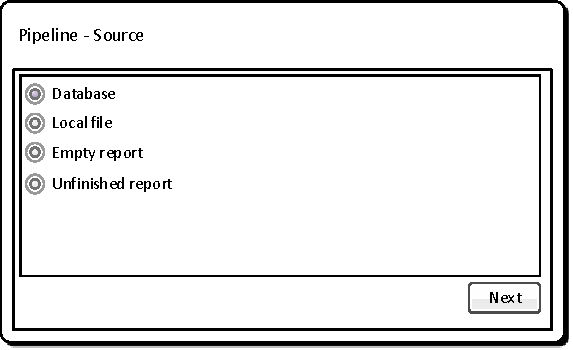
\includegraphics{Images/MockupPipelineSource}
        \caption{Selecting source of the report.}
        \label{fig:MockupPipelineSource}
\end{figure}

\begin{figure}[!htb]
        \centering
        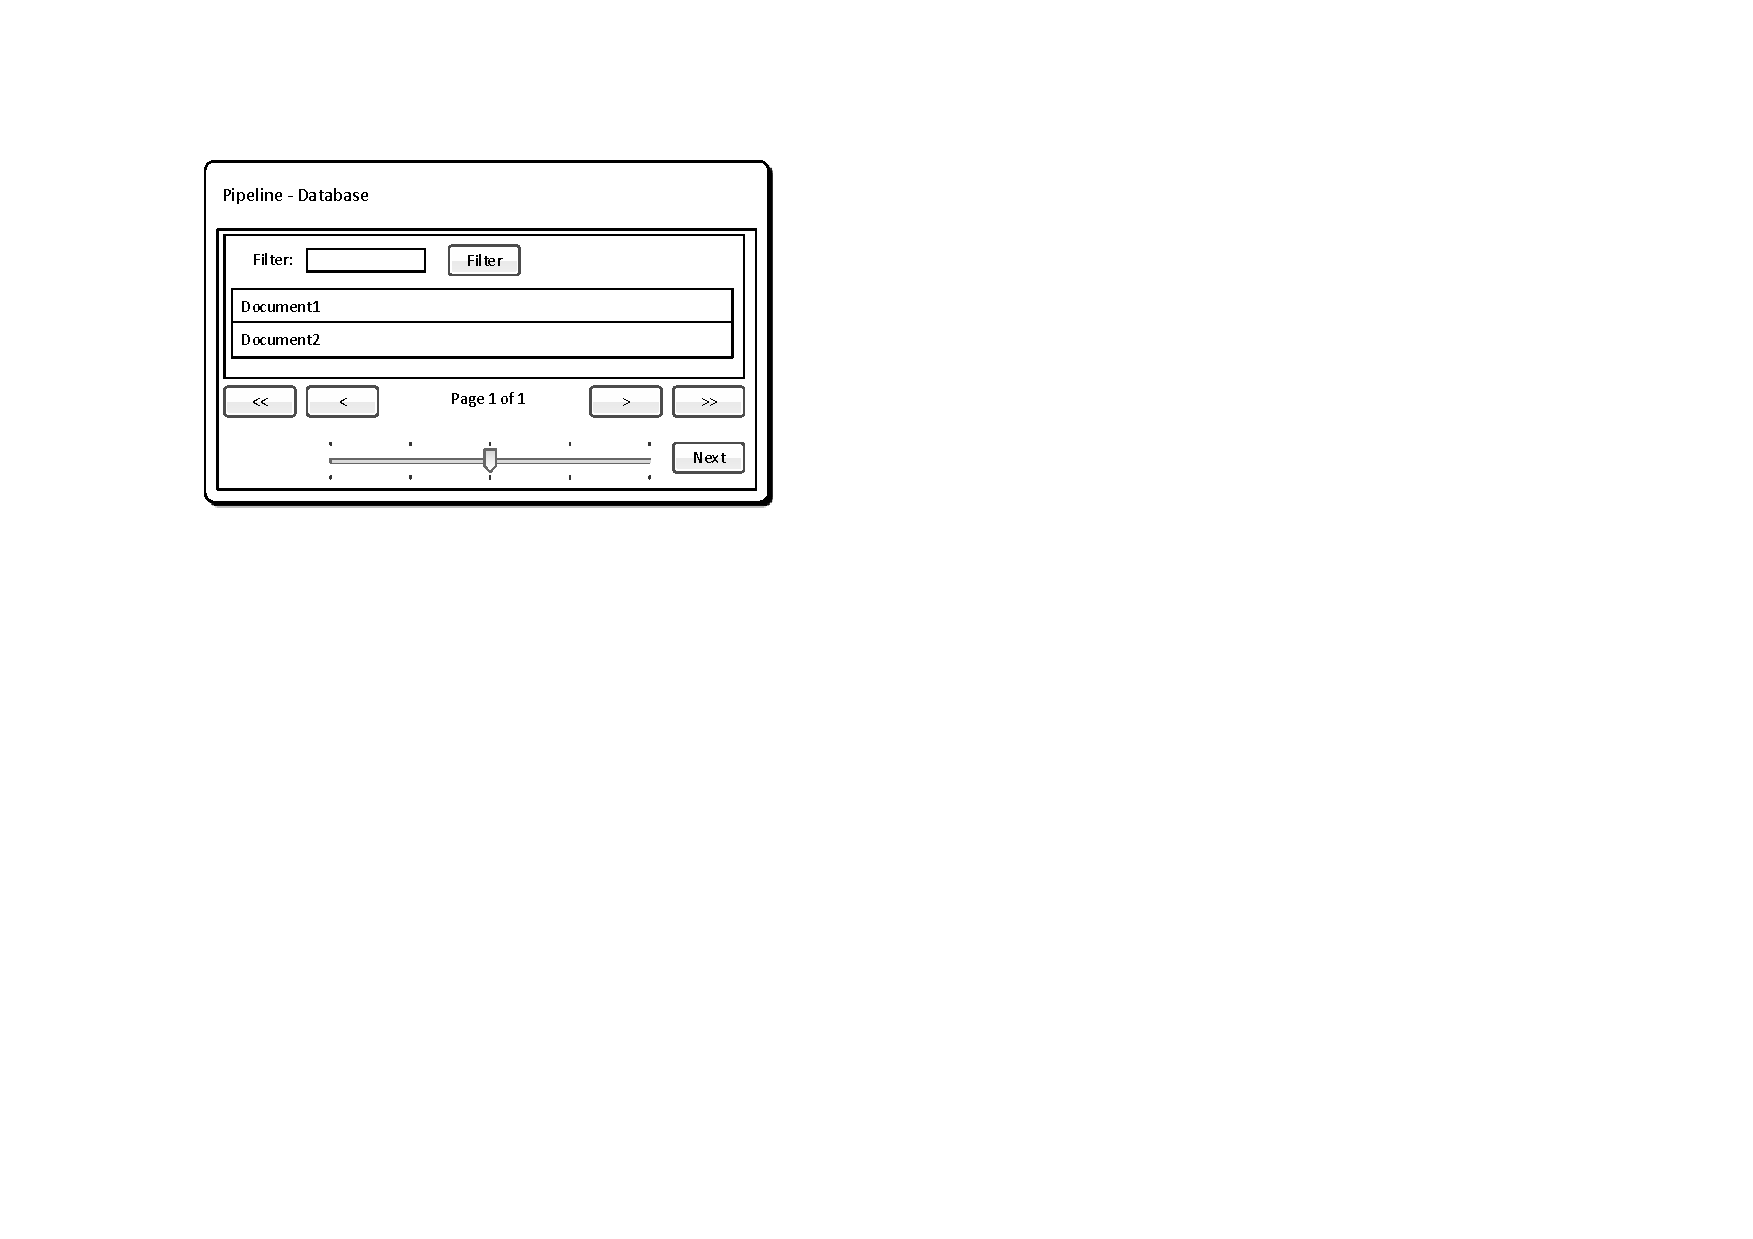
\includegraphics{Images/MockupPipelineDatabase}
        \caption{Selecting source of the report.}
        \label{fig:MockupPipelineDatabase}
\end{figure}

\begin{figure}[!htb]
        \centering
        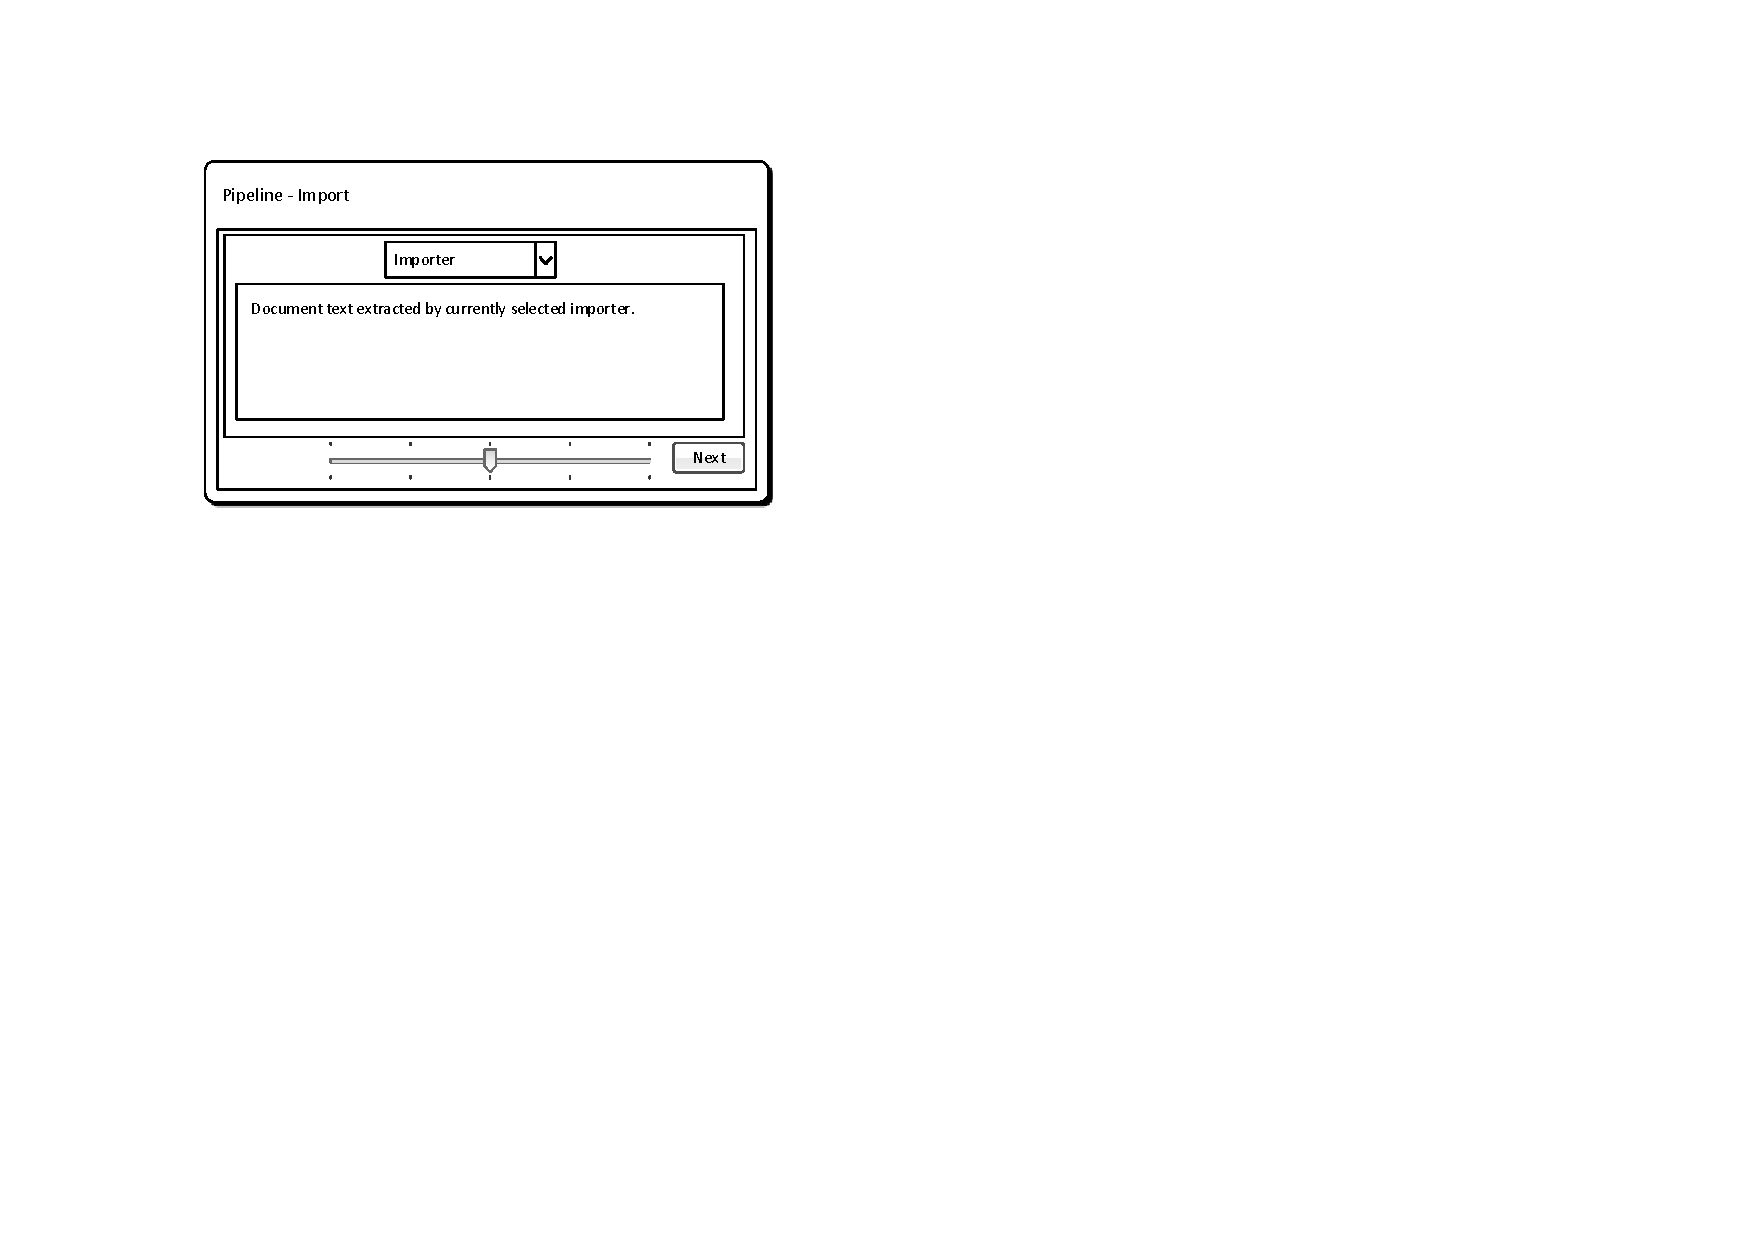
\includegraphics{Images/MockupPipelineImport}
        \caption{Importing report from a local file.}
        \label{fig:MockupPipelineImport}
\end{figure}

\begin{figure}[!htb]
        \centering
        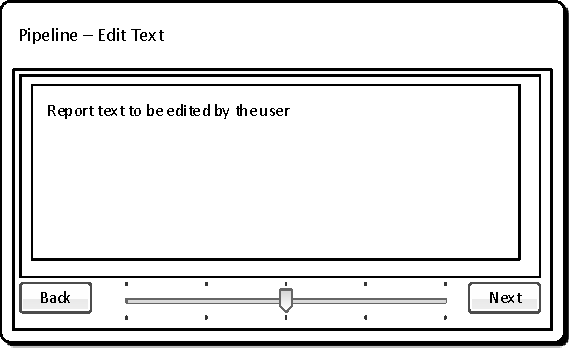
\includegraphics{Images/MockupPipelineText}
        \caption{Editing report text.}
        \label{fig:MockupPipelineText}
\end{figure}

\begin{figure}[!htb]
        \centering
        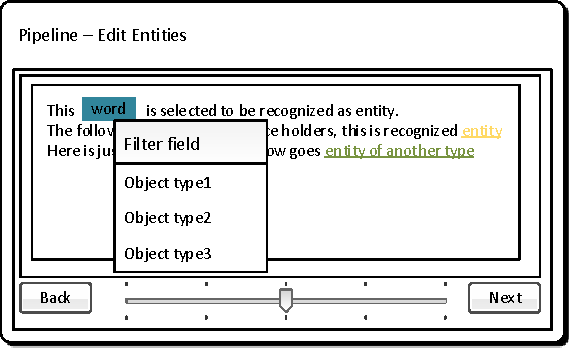
\includegraphics{Images/MockupPipelineEntities}
        \caption{Editing report entities.}
        \label{fig:MockupPipelineEntities}
\end{figure}

\begin{figure}[!htb]
        \centering
        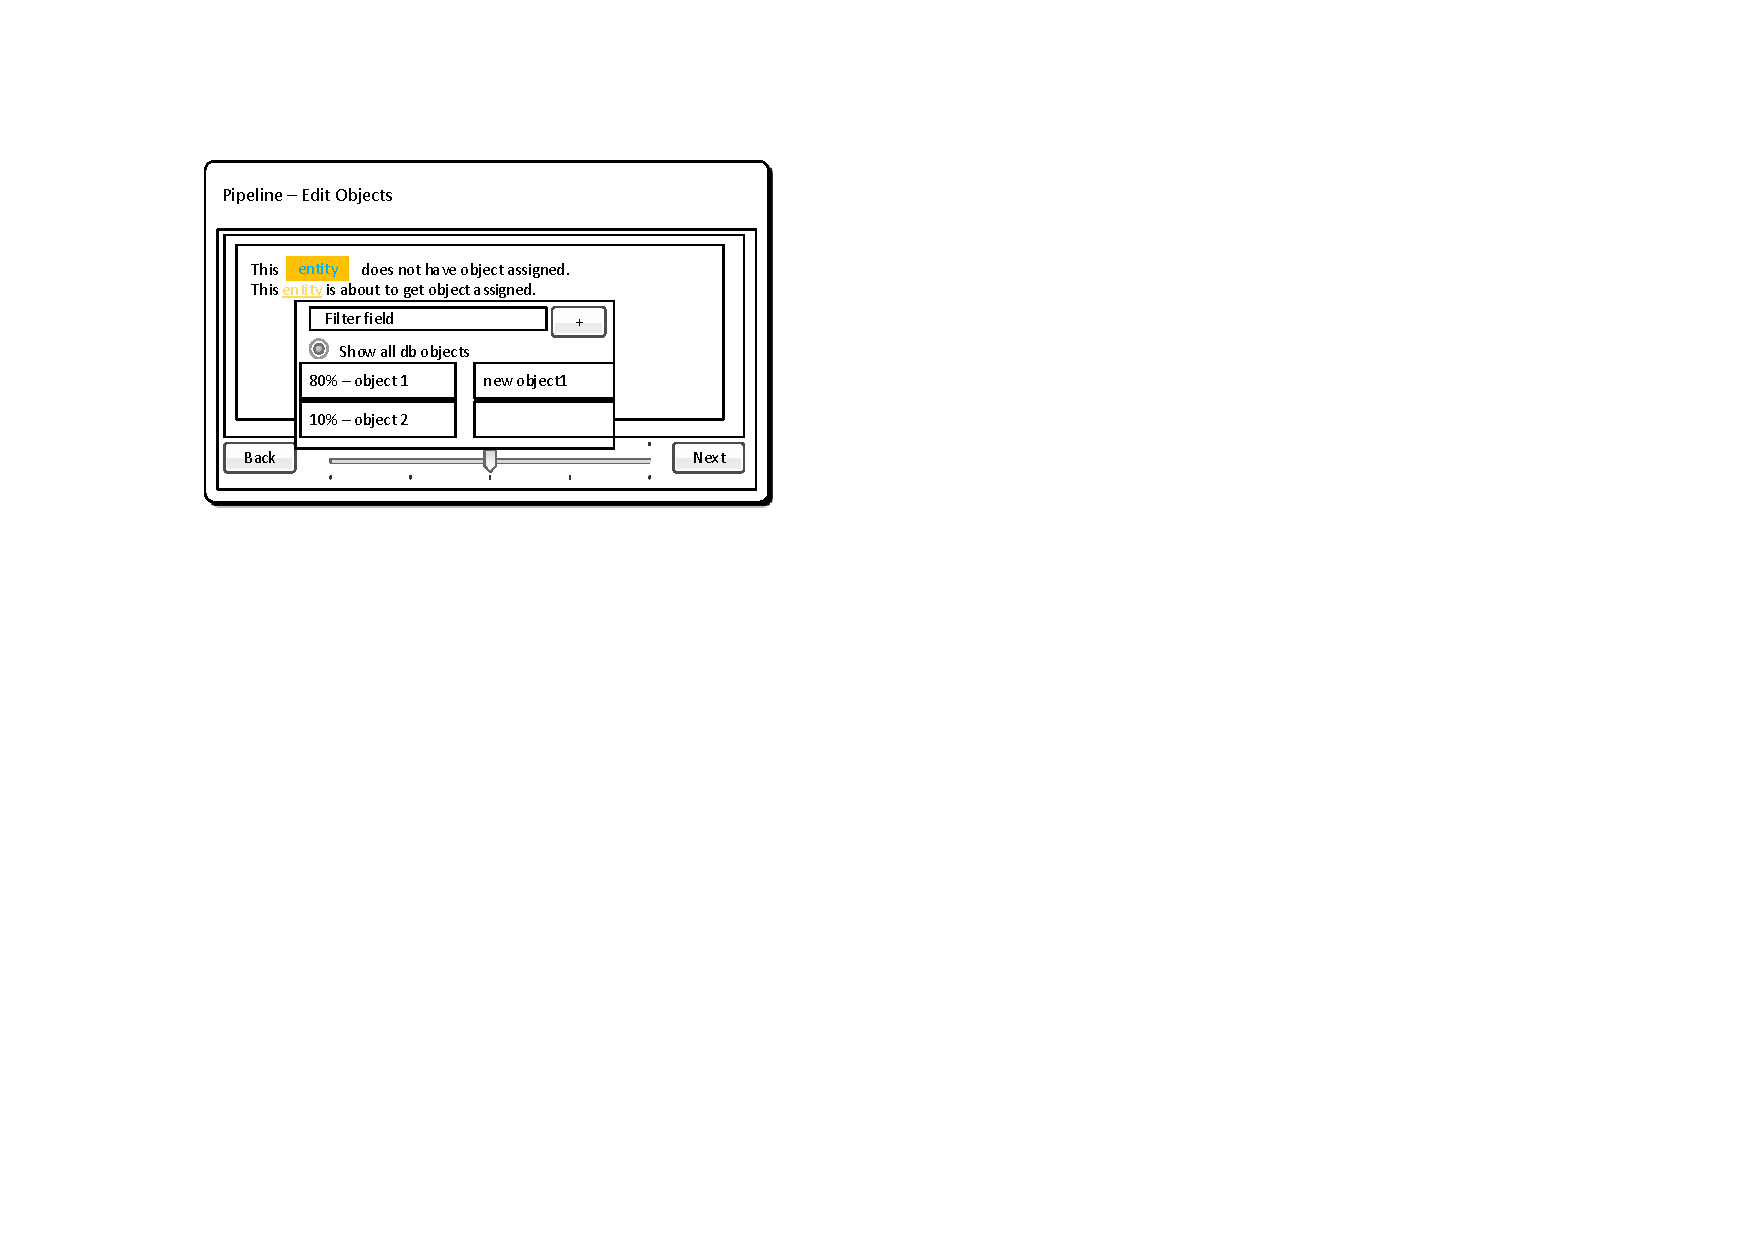
\includegraphics{Images/MockupPipelineObjects}
        \caption{Editing report objects.}
        \label{fig:MockupPipelineObjects}
\end{figure}

\begin{figure}[!htb]
        \centering
        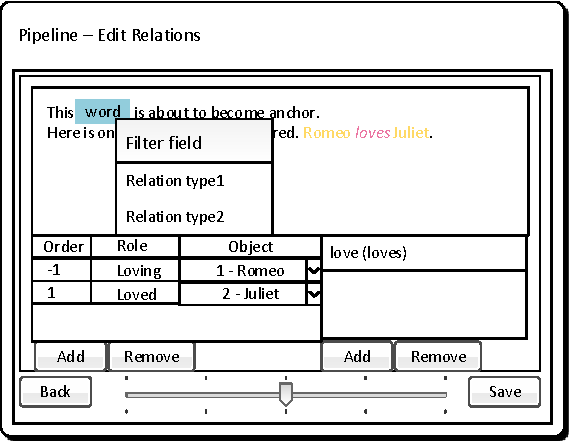
\includegraphics{Images/MockupPipelineRelations}
        \caption{Editing report relations.}
        \label{fig:MockupPipelineRelations}
\end{figure}

\begin{figure}[!htb]
        \centering
        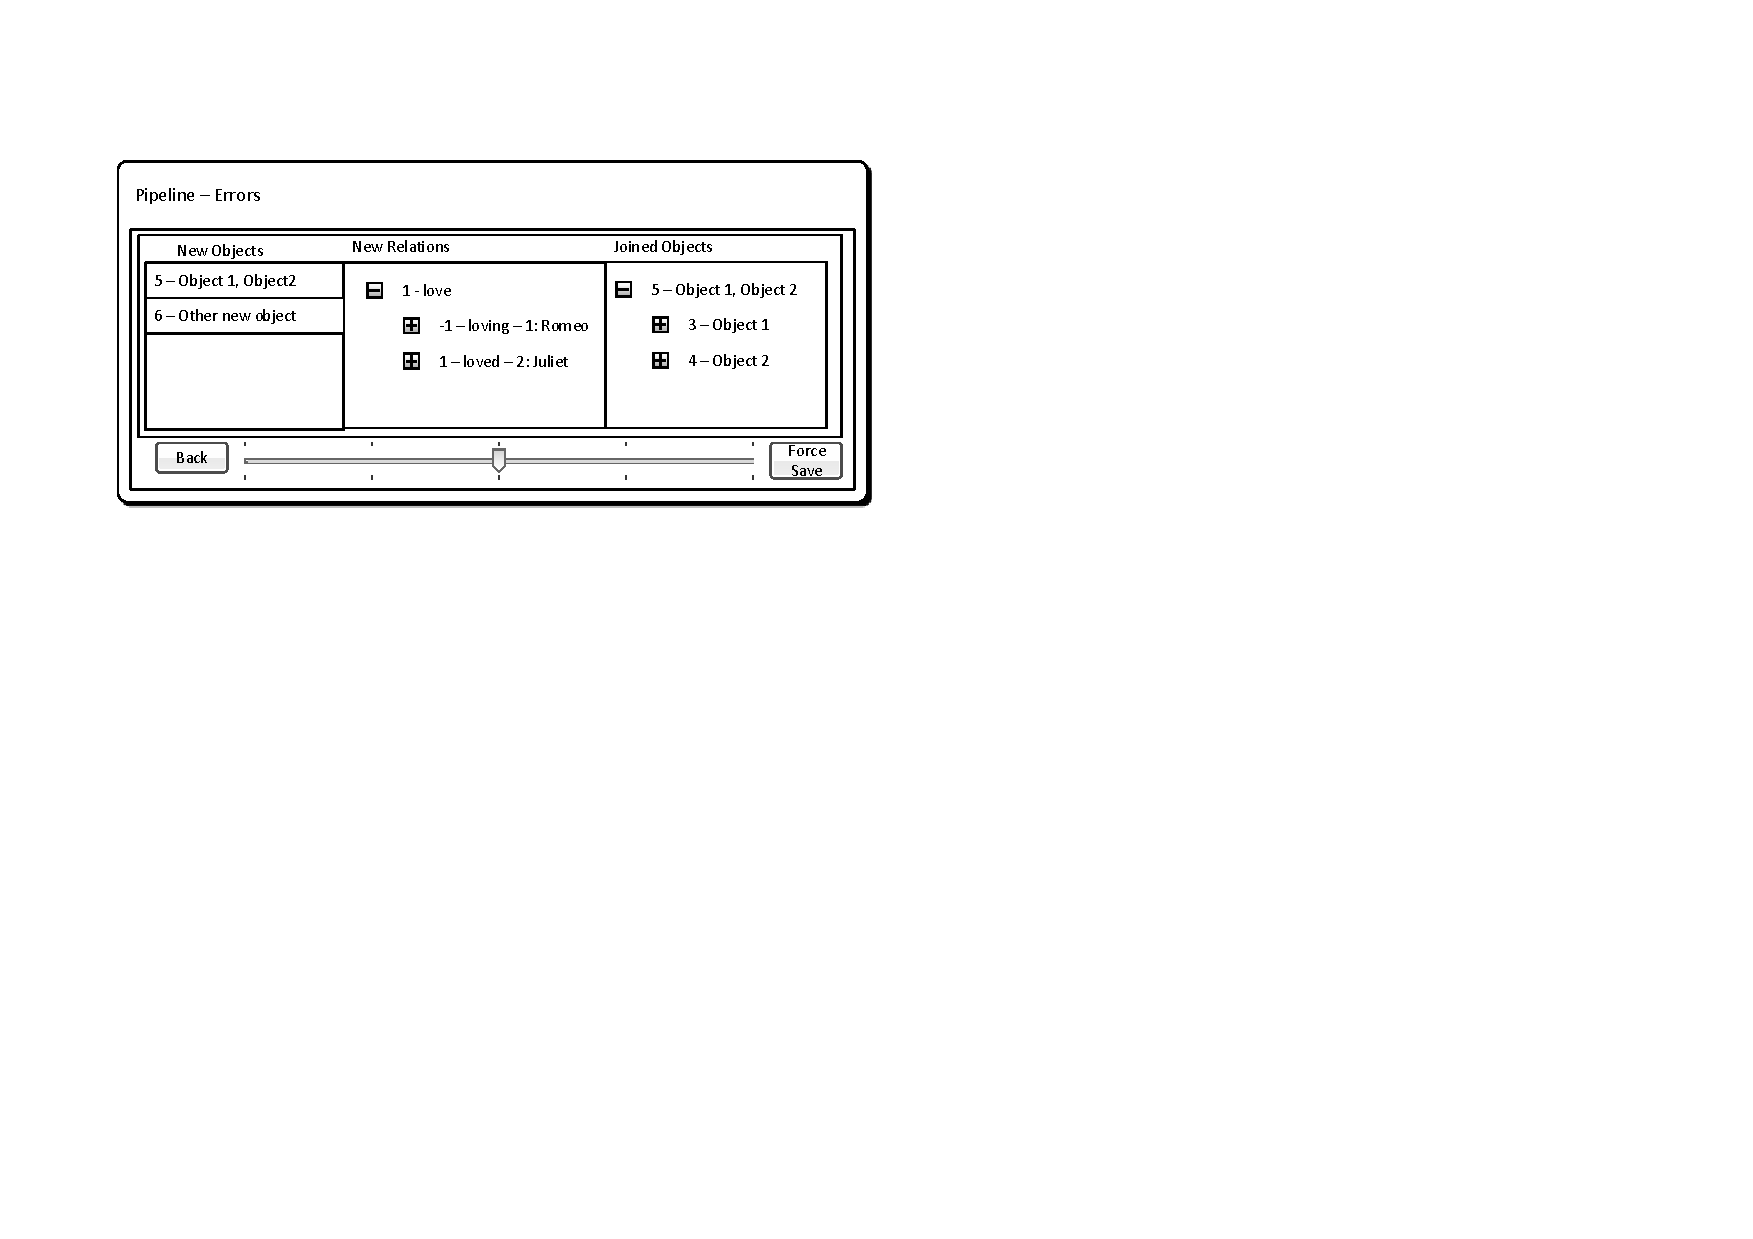
\includegraphics{Images/MockupPipelineErrors}
        \caption{Problems that may be detected on report saving.}
        \label{fig:MockupPipelineErrors}
\end{figure}

\subsection{Stateless or Stateful Communication}

\comment{Adam}{Something needs to be here!}

\subsection{Database}

First problem we had to face was choosing the type of database. As you may know
there are other databases than relational, called \emph{NoSQL} databases,
meaning \emph{Not Only SQL}. There are a few types of them, but the type that
fits the most to our problem is graph database. The standard (relational)
database is based on tables and relations between them. When you create a
database like this you have to know the exact schema and any further changes in
schema can be very hard to perform in already running system. On the other hand,
relational databases are more type safe. You just can have constraints on
columns that secure you meaningful information in the records. Graph databases
basically look like a graph - there are nodes and edges, both can have any
additional information of any kind. These are suitable especially for graph
queries that cannot be done easily in relational databases.

Anyway we decided to use the relational database for several reasons.
The graph databases are pretty new technology, it is not so time proven and we
were too afraid of possible bugs. Apart from that relational database are well
documented, all main bugs have been solved years ago and everyone knows what to
expect and what is impossible.
We also wanted to use the database for machine learning, which uses sequential
access to the database. That is, as we know, faster in relational database,
where we can only iterate through all records in a single table.
And finally none of us have an experience with graph databases.

Although we have used relational database, this decision can be proven wrong and
through the time it can come out that graph database can be much better
solution. We expected that a little bit and used the DAO design pattern enabling
to change the type of database without changing the application source code.
This pattern is more described in Section \ref{sec:PersistentLayer} about server
architecture respectively persistent layer.

This project is primary destined for policemen and their reports. They have very
a specific domain with things and people they register. We decided to create
a more general model, to enable its use and spread it into world of text
recognizers. The model is also described in details in Section\ref{sec:Database}
about the database.

\subsection{Adding New Object/Relation Types}
\label{ssec:AddingTypes}

\comment{Adam}{Explain why it is done by administrators only}

We decided that only administrators are allowed to add new object and relation
types. This is because there should be a convention used by all users that could
be ruined by uncontrolled type explosion. Limiting types manipulation should
enforce that all interventions are well thought and conceptual.
